\documentclass[aspectratio=169]{beamer}

\usetheme{default}
\setbeamertemplate{navigation symbols}{}
\setbeamertemplate{enumerate item}{\color{navy}\arabic{enumi}.}
\setbeamertemplate{itemize item}{\color{black}\textbullet}
\setbeamertemplate{itemize subitem}{\color{black}\textbullet}
\usepackage{booktabs}
\usepackage{xcolor}
\usepackage{tikz}
\usepackage{graphicx}
\usetikzlibrary{shapes,arrows,positioning}
\definecolor{navy}{RGB}{0, 0, 128}
\definecolor{lightblue}{RGB}{230,240,250}
\definecolor{darkgreen}{RGB}{0,100,0}
\definecolor{lightgreen}{RGB}{230,250,230}
\newcommand{\highlight}[1]{\colorbox{lightblue}{$\displaystyle\textcolor{navy}{#1}$}}
\newcommand{\highlighttext}[1]{\colorbox{lightblue}{\textcolor{navy}{#1}}}
\newcommand{\highlightgreen}[1]{\colorbox{lightgreen}{$\displaystyle\textcolor{darkgreen}{#1}$}}

\usepackage{hyperref}
\hypersetup{
    colorlinks=true,
    linkcolor=navy,
    urlcolor=navy,
    citecolor=navy
}

\begin{document}

\begin{frame}

\begin{center}
\Large What are proxy variables?
\end{center}

\bigskip{}

\begin{center}
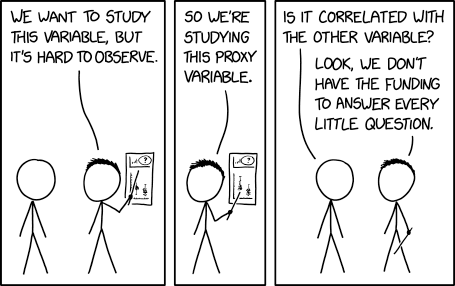
\includegraphics[width=0.5\textwidth]{proxy_variable.png}
\end{center}

\bigskip{}

\begin{center}
\small Source: \url{https://xkcd.com/2652/}
\end{center}

\end{frame}

\begin{frame}

Suppose we have a simple linear regression model

\begin{align*}
y &= X\beta + \varepsilon
\end{align*}

\begin{itemize}
\itemsep1.5em
\item<2-> In observational data, $X$ may be correlated with unobserved factors inside $\varepsilon$
\item<3-> Then OLS is biased because $\text{Cov}(X,\varepsilon) \neq 0$ (omitted variable bias)
\item<4-> One way to reduce this bias is to include a \textcolor{navy}{proxy variable}
\item<5-> A proxy is an observed variable correlated with an unobserved confounder
\item<6-> Under certain conditions, a proxy can \textcolor{navy}{reduce or even eliminate} the bias
\item<7-> e.g. IQ a proxy for unobserved ability that biases returns to schooling \end{itemize}

\end{frame}





\begin{frame}

\begin{itemize}
\itemsep1.5em
\item<1-> Proxies are often imperfect: we rarely measure the confounder exactly
\item<2-> Suppose our proxy $P$ measures the true confounder $Z$ with error:
\[
P = Z + \nu, \quad \text{Cov}(Z,\nu)=\text{Cov}(X,\nu)=0
\]
\item<3-> This is the ``classical measurement error'' (CEV) case
\item<4-> OLS estimates are \textcolor{navy}{attenuated toward zero} (``attenuation bias'')
\item<5-> Intuition: noise in the proxy dilutes the true signal
\item<6-> In non-linear models or if CEV fails, the bias can go in any direction
\item[]<6->
\begin{itemize}
    \item<7-> ``non-classical measurement error''
\end{itemize}
\end{itemize}

\end{frame}




\begin{frame}
\begin{itemize}
\itemsep1.5em
\item<1-> Unless they happen to resolve the endogeneity problem, proxy variables won't work
\item<2-> (We'd need $\mathbb{E}\left(\varepsilon \mid X, P\right) = \mathbb{E}\left(\varepsilon \mid P\right)$)
% "So what does this condition really mean? It's asking whether our proxy is **complete enough**. Once we control for P, is X basically as good as randomly assigned? Or are there still unobserved confounders linking X to the outcome? If IQ doesn't capture motivation, family networks, or other ability dimensions, then even after controlling for IQ, education choices remain correlated with unobserved determinants of wages—and we still have bias."
\item<3-> And usually proxies don't satisfy this requirement
\item<4-> You can use instrumental variables to solve the ME problem
\item<5-> But mainly in linear models
\item<6-> And, of course, instrument validity is almost always in question
\item<7-> So it seems we face a trade-off between OVB and attenuation bias
\end{itemize}
\end{frame}




\begin{frame}
\begin{itemize}
\itemsep1.5em
\item<1-> What if we have many correlated proxies?
\item<2-> For the unobserved ability question, we might have many different proxies
\item<3-> e.g. individuals might take multiple standardized tests
\item<4-> How do we know which test scores to attempt to use as proxies?
\item<5-> What if each test itself suffers from measurement error?
\item<6-> What if the test scores are highly correlated with each other?
\end{itemize}
\end{frame}

\end{document}